\documentclass[preprint,numbers]{sigplanconf}
% The following \documentclass options may be useful:

% preprint      Remove this option only once the paper is in final form.
% 10pt          To set in 10-point type instead of 9-point.
% 11pt          To set in 11-point type instead of 9-point.
% authoryear    To obtain author/year citation style instead of numeric.
\usepackage[utf8]{inputenc}          % UTF-8 Encoding
\usepackage[british]{babel}          % Use British English language settings
\usepackage{hyperref}                % Interactive PDF
\usepackage{xcolor}                  % Colours
\usepackage[inline]{enumitem}        % Inline enumerations
\usepackage{drawstack}               % Syntactic sugar for tikz for drawing run-time stacks
\usepackage{listings}                % Source code listings

\lstset{
 backgroundcolor=\color{white},   % choose the background color; you must add \usepackage{color} or \usepackage{xcolor}
 basicstyle=\ttfamily\footnotesize,        % the size of the fonts that are used for the code
 keywordstyle=\bfseries,
 commentstyle=\itshape,
 breakatwhitespace=true,         % sets if automatic breaks should only happen at whitespace
 breaklines=true,                 % sets automatic line breaking
 captionpos=b,                    % sets the caption-position to bottom
 escapeinside={\#*}{*\#},          % if you want to add LaTeX within your code
 extendedchars=true,              % lets you use non-ASCII characters; for 8-bits encodings only, does not work with UTF-8
 frame=none,	                   % adds a frame around the code
 keepspaces=true,                 % keeps spaces in text, useful for keeping indentation of code (possibly needs columns=flexible)
 numbers=none,                    % where to put the line-numbers; possible values are (none, left, right)
 rulecolor=\color{black},         % if not set, the frame-color may be changed on line-breaks within not-black text (e.g. comments (green here))
 showspaces=false,                % show spaces everywhere adding particular underscores; it overrides 'showstringspaces'
 showstringspaces=false,          % underline spaces within strings only
 showtabs=false,                  % show tabs within strings adding particular underscores
 tabsize=1,	                   % sets default tabsize to 2 spaces
 title=\lstname,                   % show the filename of files included with \lstinputlisting; also try caption instead of title
 caption={},
 belowcaptionskip=-1\baselineskip,
 xleftmargin=0.1\parindent,
 columns=fullflexible
}

% Define Links as a lst-language
\lstdefinelanguage{Links}{%
  morekeywords={typename, fun, op, var, if, true, false, else, case, switch, handle, handler, shallowhandler, do, sig},%
  sensitive=t, %
  keywordstyle=\color{red},
  emph={Comp,Bool,Int,Char,String,Choose,Return,Toss,Heads,Tails,Nothing,Just,Fail,Zero,Maybe},
  emphstyle={\color{blue}},
  comment=[l]{\#},%
  escapeinside={(*}{*)},%
  morestring=[d]{"}%
}

\newcommand{\textapprox}{{\fontfamily{ptm}\selectfont\texttildelow}}
\newcommand{\wildarrow}{\linksify{\textapprox{}>}}
% Links style
\lstdefinestyle{links}{
  basicstyle=\linespread{1.0}\ttfamily\footnotesize,
  language=Links,
  literate= {~>}{{\wildarrow}}1
}

\lstset{style={links}}

%% TODOs and comments
\newcommand{\msgbox}[2]{{%
  \par\noindent\small\color{red}%
  \framebox{\parbox{\dimexpr\linewidth-2\fboxsep-2\fboxrule}{\textbf{#1:} #2}}%
}}
\newcommand{\todo}[1]{\msgbox{TODO}{#1}}

\newcommand{\sam}[1]{\msgbox{Sam}{#1}}
\newcommand{\dhil}[1]{\msgbox{Daniel}{#1}}
\newcommand{\kc}[1]{\msgbox{KC}{#1}}

\begin{document}
%% Remove SIGPLANCONF copyright space
\makeatletter
\def\@copyrightspace{\relax}
\makeatother

%% Set paper geometry
\special{papersize=8.5in,11in}
\setlength{\pdfpageheight}{\paperheight}
\setlength{\pdfpagewidth}{\paperwidth}

%% Obfuscate e-mail addresses
\newcommand{\camacuk}{@cam.ac.uk}
\newcommand{\edacuk}{@ed.ac.uk}
\newcommand{\contact}[2]{#1@#2}
\newcommand{\reachme}[1]{\hyperlink{mailto:\contact{#1}}{\contact{#1}}}

\titlebanner{DRAFT}    % These are ignored unless
\preprintfooter{} % 'preprint' option specified.

\title{Towards Compilation of Affine Algebraic Effect Handlers}
\subtitle{-- Extended Abstract --}
\authorinfo{Daniel Hillerström}
           {The University of Edinburgh}
           {~}%{\reachme{daniel.hillerstrom}}

\authorinfo{Sam Lindley}
           {The University of Edinburgh}
           {~}%{\reachme{sam.lindley}}

\authorinfo{KC Sivaramakrishnan}
           {The University of Cambridge}
           {~}

\maketitle

\begin{abstract}
  Algebraic effects and handlers provide a modular abstraction for
  effectful programming that allow programmers to separate effect
  signatures from their implementation. We present a compiler for the
  experimental language Links with effect handlers.
\dhil{TODO: Mention the OCaml backend}

\end{abstract}

\section{Motivation}
Algebraic effects and effect handlers \cite{Plotkin2013} afford a
modular and structured interface for programming with delimited
continuations.
\dhil{TODO: Motivation regarding the efficiency of handlers.}

\kc{The paper as it stands now does not mention why, but only deals with the
question of how. We should mention the current Links backends, and say they
they are only interpreted. The goal of the project is to add support for
natively compiled backend for Links through Multicore OCaml, but also take
advantage of multicore support and efficient JS compilation that will come for
free by targetting multicore OCaml}.

Previous work focuses mostly on the design and abstraction of
handlers, but recent work has begun exploring efficient
implementations of handlers. Some notable mentions are the OCaml
Multicore project \cite{Dolan2015}, \citet{Kammar2013} embedding in
Haskell, \citet{Kiselyov2015} \emph{freer monad} implementation in
Haskell, and \citet{Wu2015} fusion optimisation for (deep) handlers.

\section{Affine and multi-shot effect handlers}
An algebraic effect is given by a signature of \emph{abstract
  operations}. For example \emph{nondeterminism} is an algebraic
effect that is given by a nondeterministic choice operation called
\lstinline$Choose$. In Links, we may use this operation to implement a
coin toss:
\begin{lstlisting}
sig toss : Comp({Choose:Bool |e}, Toss)
fun toss() { if (do Choose) Heads else Tails }
\end{lstlisting}
This declares an \emph{abstract computation} \lstinline$toss$, which
invokes an operation \lstinline$Choose$ using the \lstinline$do$
primitive.  The \lstinline$sig$ keyword begins a signature, which
reads: \lstinline$toss$ is a computation with effect signature
\lstinline${Choose:Bool |e}$ and return value \lstinline$Toss$, whose
constructors are \lstinline$Heads$ and \lstinline$Tails$.  Links
employs row typing to support extensible effect signatures, thus
\lstinline$e$ is an effect variable, which can be instantiated with
additional operations.

Introduction of another operation causes the effect signature to grow
accordingly. For example, if we introduce an exception operation
\lstinline$Fail : Zero$, then we can model a drunk coin toss:
\begin{lstlisting}
sig drunkToss : Comp({Choose:Bool,Fail:Zero |e}, Toss)
fun drunkToss() { if (do Choose) toss()
                  else switch (do Fail) { } }
\end{lstlisting}
Here \lstinline$Zero$ is the empty type, therefore the empty
\lstinline$switch$ pattern matching construct is required in order to
make the branches type check.

An effect handler instantiates a subset of the operations of an
abstract computation. For example, the following handler interprets
\lstinline$Choose$ randomly:
\begin{lstlisting}
sig randomResult : (Comp({Choose:Bool |e}, a)) ->
                    Comp({Choose{_}   |e}, a)
handler randomResult {
  case Return(x) -> x
  case Choose(k) -> k(random() > 0.5)
}
\end{lstlisting}
The signature conveys that the handler interprets the operation
\lstinline$Choose$ and leaves potentially other operations
abstract. The notation \lstinline$Choose{_}$ denotes that the
operation is polymorphic in its presence.  The handler comprises two
clauses:
\begin{enumerate*}[label={\roman*)}]
\item the \lstinline$Return$-clause specifies how to handle the return
  value of the computation.
\item the parameter \lstinline$k$ in the \lstinline$Choose$-clause is
  the (delimited) continuation of the operation \lstinline$Choose$ in the
  computation.
\end{enumerate*}
We say that \lstinline$randomResult$ is a \emph{linear handler}, because
it invokes every continuation exactly once.

Alternatively, we may give an interpretation of \lstinline$Choose$
that enumerates every possible outcome by invoking the continuation
twice:
\begin{lstlisting}
sig allResults : (Comp({Choose:Bool |e},  a)) ->
                  Comp({Choose{_}   |e}, [a])
handler allResults {
  case Return(x) -> [x]
  case Choose(k) -> k(true) ++ k(false)
}
\end{lstlisting}
Observe that the return value gets lifted into a singleton list. The
\lstinline$Choose$-clause concatenates the outcomes obtained by
interpreting the operation as \lstinline$true$ and \lstinline$false$,
respectively. We say that \lstinline$allResults$ is a \emph{multi-shot
  handler}.

Finally, we may have handlers that do not invoke continuations. These
handlers are familiarly known as \emph{exception handlers}. As an
example consider the following handler, which returns
\lstinline$Just$ the result of the computation or returns
\lstinline$Nothing$ if the operation \lstinline$Fail$ is performed:
\begin{lstlisting}
sig maybeResult : (Comp({Fail:Zero |e},       a)) ->
                   Comp({Fail{_}   |e}, Maybe(a))
handler maybeResult {
  case Return(x) -> Just(x)
  case Fail(_)   -> Nothing
}
\end{lstlisting}
The type system prevents invocation of the continuation in the an
\lstinline$Fail$-clause, because the type \lstinline$Zero$ has zero
inhabitants. Linear and exception handlers constitute \emph{affine
  handlers}.

\kc{This section is too long. Can we make this section into a background one,
where we introduce Links (mention handlers, row polymorphism, effect system)
and also introduce OCaml's effect handlers (efficient, direct-style
implementation of continuations i.e, not CPS but heap-managed stack
datastructure). Mention that OCaml provides one-shot affine handlers with the
option of explicitly cloning them. Do also mention that OCaml does not have
effect typing.}

\section{Compiler infrastructure}
\dhil{OCaml run-time maintains a stack of handlers; no optimisations.}
\kc{Mention that the compilation strategy targets OCaml's Lambda intermediate
code. Mention the reasons behind this choice, which seems unintuitive to a
casual reader. The reason being that fundamentally, Links' type-system is more
expressive than OCaml's (row-polymorohism) and hence Links programs cannot be
faithfully translated to surface OCaml syntax. By targetting Lambda, we subvert
OCaml's typechecker, but since the Links programs are typechecked already, the
translation is safe.}

OCaml supports only affine handlers. Multiple invocations of a continuation
causes a run-time error.  In contrast to OCaml, our implementation supports
multi-shot handlers. In fact, we use \lstinline$Obj.clone$ to encode multi-shot
handlers. \kc{$Obj.clone$ was too generic and I plan to use
$Obj.clone\_continuation$ to be less ambiguous.}
\begin{figure}
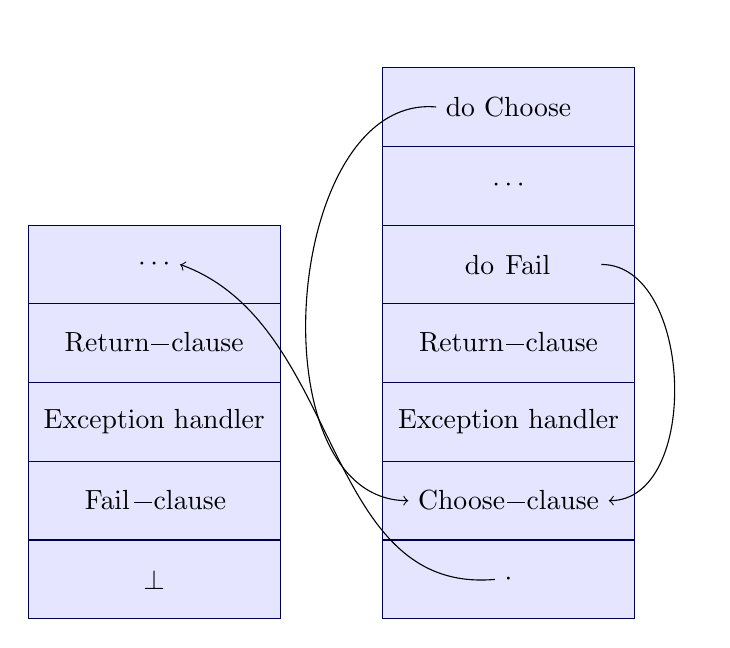
\begin{tikzpicture}
  \drawstruct{(4.5,2)}
  \structcell{\lstinline$do Choose$}  \coordinate (DoChoose) at (currentcell.west);
  \structcell{$\cdots$}
  \structcell{\lstinline$do Fail$} \coordinate (DoFail) at (currentcell.east);
  \structcell{\lstinline$Return-clause$}
  \structcell{\lstinline[keywordstyle=\footnotesize]$Exception handler$}
  \structcell{\lstinline$Choose-clause$} \coordinate (HandleChoose1) at (currentcell.west); \coordinate (HandleChoose2) at (currentcell.east);
  \structcell{$\cdot$} \coordinate (H1) at (currentcell.west);

  \drawstruct{(0,0)}
  \structcell{$\cdots$} \coordinate (H2) at (currentcell.east);
  \structcell{\lstinline$Return-clause$}
  \structcell{\lstinline[keywordstyle=\footnotesize]$Exception handler$}
  \structcell{\lstinline$Fail-clause$}
  \structcell{$\bot$}

%  \draw[<-] (H2) .. controls ([yshift=0cm] H2) and ([xshift=-10cm,yshift=4cm] H1) .. (H1);
  \draw (H2) edge[out=-20,in=-175,<-] (H1);
  \draw (DoChoose) edge[out=175,in=-180,->] (HandleChoose1);
  \draw (DoFail) edge[xshift=0.5cm,out=0,in=-360,->] (HandleChoose2);
\end{tikzpicture}
\caption{Runtime representation of the computation \lstinline$maybeResult(randomResult(drunkToss))$.}\label{fig:rtstack}
\end{figure}

\section{Optimisations}
It is rather conservative to implement every handler as multi-shot. We
would like to recover the efficiency of affine handlers.
\kc{Even without the optimizations, I expect Links compiled to OCaml to be
faster than the interpreted version. Compare the performance on Queens? By
varying the board size:
https://github.com/kayceesrk/ocaml-eff-example/blob/master/queens.ml}

\paragraph{Linearisation}
It is well-known that linear continuations have efficient
representations \cite{Bruggeman1996}.  We use Links' linear type
system to track the linearity of handlers. This enable us to
specialise the implementation of handlers during code generation.

% \paragraph{Fusion} Handler fusion is a technique to prune the run-time
% stack. Consider the composition
% \lstinline$maybeResult(randomResult(toss))$. It gives
% rise to a stack with two handlers.  We may use row types to guide when
% handler fusion is sound. A necessary criterion for fusion of two
% handlers is that the intersection of their effect signatures is
% empty. We fuse handlers clause by clause, thus for
% \lstinline$maybeResult$ and \lstinline$randomResult$ we obtain:
% \begin{lstlisting}
% sig fused : (Comp({Choose:Bool,Fail:Zero |e}, a)) ->
%              Comp({Choose{_}  ,Fail{_}   |e}, Maybe(a))
% handler fused {
%   case Return(x) -> var y = x; Just(y)
%   case Fail(_)   -> Nothing
%   case Choose(k) -> k(random() > 0.5)
% }
% \end{lstlisting}

% \paragraph{Inlining} Operation inlining enables us to replace abstract
% operations with their implementations, when these are statically
% resolvable. Furthermore, the handler must affine and the operation
% clause must invoke the continuation in tail position. For example, in
% the application \lstinline$randomResult(toss)$ we may replace
% \lstinline$do Choose$ with the computation \lstinline$random() > 0.5$ at compile-time.

\section{Acknowledgements}
The first author was supported by EPSRC CDT in Pervasive Parallelism
(grant EP/L01503X/1).  The second author was supported by EPSRC grant
number EP/K034413/1.  Thanks to OCaml Labs\dots

\bibliographystyle{abbrvnat} \softraggedright
\bibliography{references}

\end{document}
